% cSpell: disable
\section{Deep Learning}

\begin{frame}[plain,c]
    %\frametitle{A first slide}

    \begin{center}
        \color{DarkBlue}
    \Huge \thesection. \insertsection
    \end{center}

\end{frame}

\begin{frame}{The power of Deep Learning}
    % we want to learn a complicated function that tells us whether an image is an MR image
    % similarly deep learning has been able to build functions that tell whether an image is that of a dog or a cat
    % universal approx
    % We want to learn a complicated function that tells us whether a complex-valued vector is an MR image or not.
    % We want a function that tells us whether a vector is an MR image or not.
    The prior is a complicated visual function.
    \pause

    Deep Learning~(DL) has been used to build complicated functions:
    {\Large
        \begin{equation*}
            \tikzmarknode{nn}{\highlight{brown}{$f_\thetab$}}\left( \adjincludegraphics[valign=c,width=0.2\textwidth]{Figures/intro_figures/chowchow.jpg} \right) = \text{"DOG"}
        \end{equation*}
        \begin{tikzpicture}[overlay,remember picture,>=stealth,nodes={align=left,inner ysep=1pt},<-,font=\normalsize]
            % For "nn"
            \onslide<3->{
            \path (nn.south) ++ (0, -4.5em) node[anchor=south west,color=brown!87] (exp_nn){
                Neural network:\\a chain of elementary linear \& nonlinear functions};
            \draw [color=brown!87](nn.south) |- ([xshift=-0.3ex,color=brown]exp_nn.south east);
            }
        \end{tikzpicture}
    }
\end{frame}

\begin{frame}{Formalism - 1}
    % supervised learning objective function
    % The classical framework for DL is supervised learning:
    Supervised learning:
    \vspace{\baselineskip}

    \begin{equation*}
        \argmin_{\tikzmarknode{params}{\highlight{orange}{$\thetab \in \Theta$}}} \tikzmarknode{sum}{\highlight{purple}{$\sum\limits_{(\xb_i, \yb_i) \in \mathcal{D}}$}} \tikzmarknode{loss}{\highlight{green}{$\mathcal{L}$}}(\tikzmarknode{nn}{\highlight{brown}{$f_{\thetab}$}} (\tikzmarknode{input}{\highlight{blue}{$\xb_i$}}), \tikzmarknode{label}{\highlight{red}{$\yb_i$}}, \thetab)
    \end{equation*}
    % XXX add visual aid to formalism
    \begin{tikzpicture}[overlay,remember picture,>=stealth,nodes={align=left,inner ysep=1pt},<-]
        % For "input"
        \onslide<2->{
        \path (input.north) ++ (0,1.5em) node[anchor=south west,color=blue!87] (exp_input){
            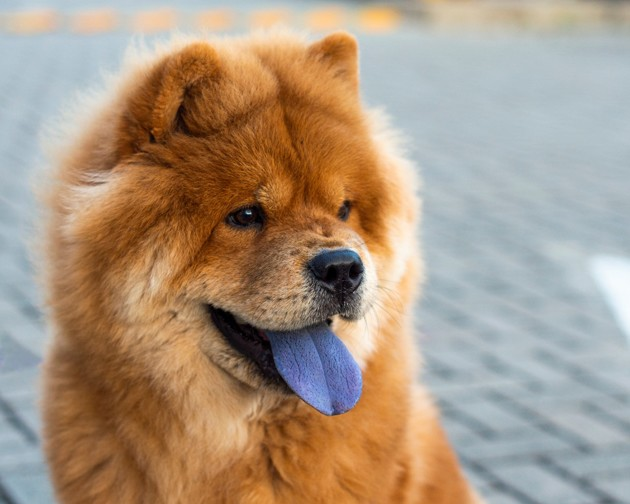
\includegraphics[width=0.05\textwidth]{Figures/intro_figures/chowchow.jpg} input};
        \draw [color=blue!87](input.north) |- ([xshift=-0.3ex,color=blue]exp_input.south east);
        }
        % For "label"
        \onslide<3->{
        \path (label.south) ++ (0, -2.5em) node[anchor=south west,color=red!87] (exp_label){
            "DOG", label};
        \draw [color=red!87](label.south) |- ([xshift=-0.3ex,color=red]exp_label.south east);
        }
        % For "nn"
        \onslide<4->{
        \path (nn.south) ++ (0, -4.5em) node[anchor=south east,color=brown!87] (exp_nn){
            neural network};
        \draw [color=brown!87](nn.south) |- ([xshift=-0.3ex,color=brown]exp_nn.south west);
        }
        % For "loss"
        \onslide<5->{
        \path (loss.north) ++ (0, 1.5em) node[anchor=south west,color=DarkGreen!77] (exp_loss){
            loss};
        \draw [color=DarkGreen!87](loss.north) |- ([xshift=-0.3ex,color=DarkGreen]exp_loss.south east);
        }
        % For "sum"
        \onslide<6->{
        \path (sum.south) ++ (0, -2em) node[anchor=south east,color=purple!87] (exp_sum){
            Estimator of the expected value};
        \draw [color=purple!87](sum.south) |- ([xshift=-0.3ex,color=purple]exp_sum.south west);
        }

        % For "params"
        \onslide<7->{
        \path (params.west) ++ (-2em, 0) node[anchor=east,color=orange!87] (exp_params){
            Parameters};
        \draw [color=orange!87](params.west) -- ([xshift=-0.3ex,color=orange]exp_params.east) -- ([xshift=-0.3ex,color=orange]exp_params.south east) -- ([xshift=-0.3ex,color=orange]exp_params.south west);
        }

    \end{tikzpicture}
\end{frame}

\begin{frame}{Formalism - 2}
    % Stochastic Gradient descent and chain rule
    To solve the previous equation we will use two main tools:

    \begin{enumerate}
        \item \alt<2>{Stochastic Gradient Descent~(SGD)}{\highlight{blue}{Stochastic Gradient Descent~(SGD)}};
        \item<2> \highlight{blue}{Chain rule}.
    \end{enumerate}


        \begin{block}{Definition}
            \only<1>{An algorithm to solve the previous optimization problem based on first order derivatives.}
            \only<2>{
                A property allowing us to compute easily derivatives of compound functions.
                \begin{equation*}
                    \frac{\partial f}{\partial y} = \frac{\partial f}{\partial x} \frac{\partial x}{\partial y}
                \end{equation*}
            }
        \end{block}

\end{frame}

\begin{frame}{Requirements for Deep Learning}
    % Great that I can do that, but does it take ?
    % Data, compute + memory, framework
    % accept that it's "black-box"
    What does it take to use DL in a problem?
    \begin{itemize}[<+->]
        \item data
        \item compute \& memory
        \item development framework
        \item accepting that it's "black-box"
    \end{itemize}
\end{frame}

% \begin{frame}{Building the network}
%     % give classical functions
% \end{frame}

\begin{frame}{Introduction Recap}
    \begin{block}{Recap}
        MRI is slow because of \textbf{relaxation}.

        \pause
        If we want to do fewer relaxations, we need to exploit some \textbf{redundancy} in MR images.

        \pause
        But this redundancy is not easy to express with handcrafted linear functions.

        \pause
        This is why we want to use \textbf{Deep Learning} which enables the calibration of complicated functions.
    \end{block}
\end{frame}
